\documentclass[]{article}
\usepackage{lmodern}
\usepackage{amssymb,amsmath}
\usepackage{ifxetex,ifluatex}
\usepackage{fixltx2e} % provides \textsubscript
\ifnum 0\ifxetex 1\fi\ifluatex 1\fi=0 % if pdftex
  \usepackage[T1]{fontenc}
  \usepackage[utf8]{inputenc}
\else % if luatex or xelatex
  \ifxetex
    \usepackage{mathspec}
  \else
    \usepackage{fontspec}
  \fi
  \defaultfontfeatures{Ligatures=TeX,Scale=MatchLowercase}
\fi
% use upquote if available, for straight quotes in verbatim environments
\IfFileExists{upquote.sty}{\usepackage{upquote}}{}
% use microtype if available
\IfFileExists{microtype.sty}{%
\usepackage{microtype}
\UseMicrotypeSet[protrusion]{basicmath} % disable protrusion for tt fonts
}{}
\usepackage[margin=1in]{geometry}
\usepackage{hyperref}
\hypersetup{unicode=true,
            pdftitle={A climate selection experiment with 501 Arabidopsis thaliana genotypes},
            pdfauthor={Moises Exposito-Alonso , Rocío Gómez Rodríguez, Cristina Barragán, Oliver Bossdor, Giovana Capovila, Enyoung Chae, Jane Devos, Ezgi Dogan, Claudia Friedeman, Caspar Gross, Patricia Lang, Derek Lundberg, Belén Méndez-Vigo, Vera Middendorf, Jorge Kagayema, Talia Karasov, Sonja Kersten, Sebastian Petersen, Leily Rabani, Julian Regalado, Beth Rowan, Danelle Seymor, Efftimia Simeonidi, Rebecca Schwab, Diep Tran, Kavita Venkataramani, Anna-Lena Van de Weyer, Ronja Wedegärtner, Frank Weiss, Rui Wu, Wanyan Xi, Mari Cris Zaidem, Wansheng Zhu, Carlos Alonso Blanco, Xavier Picó, Hernán A. Burbano, Oliver Bossdorf, Detlef Weigel  correspondence to moisesexpositoalonao@gmail.com},
            pdfborder={0 0 0},
            breaklinks=true}
\urlstyle{same}  % don't use monospace font for urls
\usepackage{graphicx,grffile}
\makeatletter
\def\maxwidth{\ifdim\Gin@nat@width>\linewidth\linewidth\else\Gin@nat@width\fi}
\def\maxheight{\ifdim\Gin@nat@height>\textheight\textheight\else\Gin@nat@height\fi}
\makeatother
% Scale images if necessary, so that they will not overflow the page
% margins by default, and it is still possible to overwrite the defaults
% using explicit options in \includegraphics[width, height, ...]{}
\setkeys{Gin}{width=\maxwidth,height=\maxheight,keepaspectratio}
\IfFileExists{parskip.sty}{%
\usepackage{parskip}
}{% else
\setlength{\parindent}{0pt}
\setlength{\parskip}{6pt plus 2pt minus 1pt}
}
\setlength{\emergencystretch}{3em}  % prevent overfull lines
\providecommand{\tightlist}{%
  \setlength{\itemsep}{0pt}\setlength{\parskip}{0pt}}
\setcounter{secnumdepth}{0}
% Redefines (sub)paragraphs to behave more like sections
\ifx\paragraph\undefined\else
\let\oldparagraph\paragraph
\renewcommand{\paragraph}[1]{\oldparagraph{#1}\mbox{}}
\fi
\ifx\subparagraph\undefined\else
\let\oldsubparagraph\subparagraph
\renewcommand{\subparagraph}[1]{\oldsubparagraph{#1}\mbox{}}
\fi

%%% Use protect on footnotes to avoid problems with footnotes in titles
\let\rmarkdownfootnote\footnote%
\def\footnote{\protect\rmarkdownfootnote}

%%% Change title format to be more compact
\usepackage{titling}

% Create subtitle command for use in maketitle
\newcommand{\subtitle}[1]{
  \posttitle{
    \begin{center}\large#1\end{center}
    }
}

\setlength{\droptitle}{-2em}
  \title{A climate selection experiment with 501 \emph{Arabidopsis thaliana}
genotypes \newline}
  \pretitle{\vspace{\droptitle}\centering\huge}
  \posttitle{\par}
  \author{Moises Exposito-Alonso \textsuperscript{1}, Rocío Gómez Rodríguez,
Cristina Barragán, Oliver Bossdor, Giovana Capovila, Enyoung Chae, Jane
Devos, Ezgi Dogan, Claudia Friedeman, Caspar Gross, Patricia Lang, Derek
Lundberg, Belén Méndez-Vigo, Vera Middendorf, Jorge Kagayema, Talia
Karasov, Sonja Kersten, Sebastian Petersen, Leily Rabani, Julian
Regalado, Beth Rowan, Danelle Seymor, Efftimia Simeonidi, Rebecca
Schwab, Diep Tran, Kavita Venkataramani, Anna-Lena Van de Weyer, Ronja
Wedegärtner, Frank Weiss, Rui Wu, Wanyan Xi, Mari Cris Zaidem, Wansheng
Zhu, Carlos Alonso Blanco, Xavier Picó, Hernán A. Burbano, Oliver
Bossdorf, Detlef Weigel \newline \newline  \textsuperscript{1}
correspondence to
\href{mailto:moisesexpositoalonao@gmail.com}{\nolinkurl{moisesexpositoalonao@gmail.com}}}
  \preauthor{\centering\large\emph}
  \postauthor{\par}
  \predate{\centering\large\emph}
  \postdate{\par}
  \date{21 05 2017}


\begin{document}
\maketitle

{
\setcounter{tocdepth}{2}
\tableofcontents
}
\pagebreak

\section{Abstract}\label{abstract}

Evolution experiments with manipulated environmental variables is the
most robust approach to characterize natural selection, yet rarely it
can be done at the genomic scale. We carry out two field experiment, in
a Mediterranean and a Central European locations, with manipulated
rainfall using 520 accessions of the model plant Arabidopsis thaliana
and measure selection coefficients along the genome.

\emph{Keywords}: Arabidopsis thaliana, climate change, natural
selection, selection screen

\section{The ecotypes from the 1001 Genomes
Projects}\label{the-ecotypes-from-the-1001-genomes-projects}

The 1001 project comprises 1135 accession lines sequenced. Here are the
details of the protocol used to select the most informative, less biased
sample of the lines within the 1001 genomes project in order to
prioritize phenotypic efforts. Filtering consisted in several
approaches: (1) First we aimed to remove those accessions with the
lowest genome quality. Among 1135, we discarded those with \textless{}
10X genome coverage and \textless{} 90\% congruence of SNPs called from
Max Planck Institute and Gregor Mendel Institute pipelines (1001 Genomes
Consortium 2016). The remaining number were 959 accessions. (2)
Parallely, we filtered almost-identical individuals. Using plink we
computed identity by state genome-wide across the 1135 accessions. For
those pairs of accessions with \textless{} 0.01 differences in total
number of SNP, we randomly picked one. This resulted in 889 accessions.
The merge between (1) and (2) criteria was 762. (3) Finally, we reduced
geographic ascertainment. Sampling for the 1001g project was not
performed in neither a random nor regular structured scheme. Some
laboratories provided several lines per locations whereas others
provided lines that were at least several hundred kilometres apart.
Employing latitude and longitude degrees, we computed euclidean
distances across the 11135 accessions and identified pairs that were
\textless{} 0.0001 distance, that is accessions from the same population
( \textless{}\textless{} 100 meters), and randomly picked one. This
resulted in 682 accessions. We merged the resulting lists of accessions
after the three quality filtering procedures and obtained a final set of
523 accessions. 211 shared from other experiments, and were used here.

\section{Field experiment design}\label{field-experiment-design}

We grew xyz We used trays of 8x5 cells (5.5 x 5.5 x10cm size).

\subsection{Blocking and
randomisation}\label{blocking-and-randomisation}

We used a incomplete block randomized designed (Fig. S2).

\subsection{Removal of errors during
sowing}\label{removal-of-errors-during-sowing}

In a large field experiment enterprise errors can occur, but these
errors can be reduced by reducing the``degrees of freedom'' of the
experimenters. We tried to accomplish this by preparing and curating all
eppendorf with the seeds to be sown in cardboard boxes with the same
cells as in the target quick pots and arranged in their corresponding
(randomised) locations. Then, during sowing each experimenter took a box
at random and went to the corresponding tray in the field previously
arranged (Fig. S2). This reduced the possible errors, and those
positions were detected, were removed from the analyses.

\subsection{Considerations about
contamination}\label{considerations-about-contamination}

Because we were aware that contamination of neighboring pots was a risk.
We were extremely careful during sowing. We pick a day with no wind and
we throw the seeds from 1-2 cm height. During the vegetative grow we
identified germination that looked like neighbour contamination and
remove those. Although we lost a number of plants, the power of the
design was the replication, thus we discarded everything that looked
suspicious. During flowering recording (see section) we observed
homogeneity of flowering as a trait that could further indicate
contamination

\section{Recording of flwoering time}\label{recording-of-flwoering-time}

With a frequency of once every two or three days, we visited the field
experiment on average every 1 or 2 days and recorded what pots had
flowered. To keep track from previous visits, we sticked blue pins in
the pots were flowering was recorded. This removed a source of human
error.

\section{Image production and
analysis}\label{image-production-and-analysis}

Images for analyses are available at dryadxxx

\subsection{Vegetative rosettes}\label{vegetative-rosettes}

With a frequency varying x and x we took top-view pictures of trays
(Exposito-Alonso et al. 2017) and segmented them for green pixels
(\url{https://github.com/MoisesExpositoAlonso/hippo}, ref.
({\textbf{???}})). Data cleaning, processing and visualization is
available at:
\url{https://github.com/MoisesExpositoAlonso/field/analyses/docs/growth.html}
Employing duplicated images (same quickpot tray and same day, n=790 pot
pixel counts) we were able to calculate a replicability rate between two
identical pots of 99.6\%. We did this using a generalized random
regression of the green pixel counts (poisson family) on the pot
identity, and we calculated the percentage of variance associated to the
pot identity. In order to eliminate pots that did not germinate, during
the experiment we marked pots with red tape, easily identified by image
analysis. The distribution of the cumulative sum of red pixels is
bimodal under log-transform axis. This corresponds to pots with
essentially no large areas of red and those with large red labels (Fig.
S3). The exact threshold was established by measuring the variance
between and within the two groups of pots. The threshold that maximized
the variance between was chosen. To infer parameters about germination
and growth, we modeled the trajectories of green pixels as sigmoidal
curve from the start of the experiment (zero pixels) to the highest
value in the two first months. The three parameters were stored together
with also an analogous linear model and a We used the first day where
any green pixel could be detected (pixels had resolution of
submillimeter {[}input value{]}).

\subsection{Reproductive plants}\label{reproductive-plants}

We used Otsu's adaptive thresholding algorithm from OpenCV module to
convert three channel images into a white/black segmented picture. Then
we utilized the thin function from Mahotas module to erodes the binary
picture to a single-pixel path --- called skeletonisation. Finally, to
detect the branching points we used

\section{Additional datasets}\label{additional-datasets}

\subsection{Vasseur et al. 2017}\label{vasseur-et-al.-2017}

\subsection{Fournier-Level et al.
2011}\label{fournier-level-et-al.-2011}

\subsection{Slovak et al. 2014}\label{slovak-et-al.-2014}

\subsection{1001 Genomes Consortium 2016}\label{genomes-consortium-2016}

\subsection{Figures}\label{figures}

Figure 1. Accessions locations

Figure 2. Picture of experimental sites

\centerline{\includegraphics[width=7in]{../figs/Figure_S2_field_spatial_distribution.pdf.png}}
Figure 3. Design of field experiment foil tunnel and treatments in space

Figure 4. Example image and pixel segmentation

Figure 5. Example image and skeletonisation

\section{Author contributions}\label{author-contributions}

The detailed list of contributed tasks of each authors

\centerline{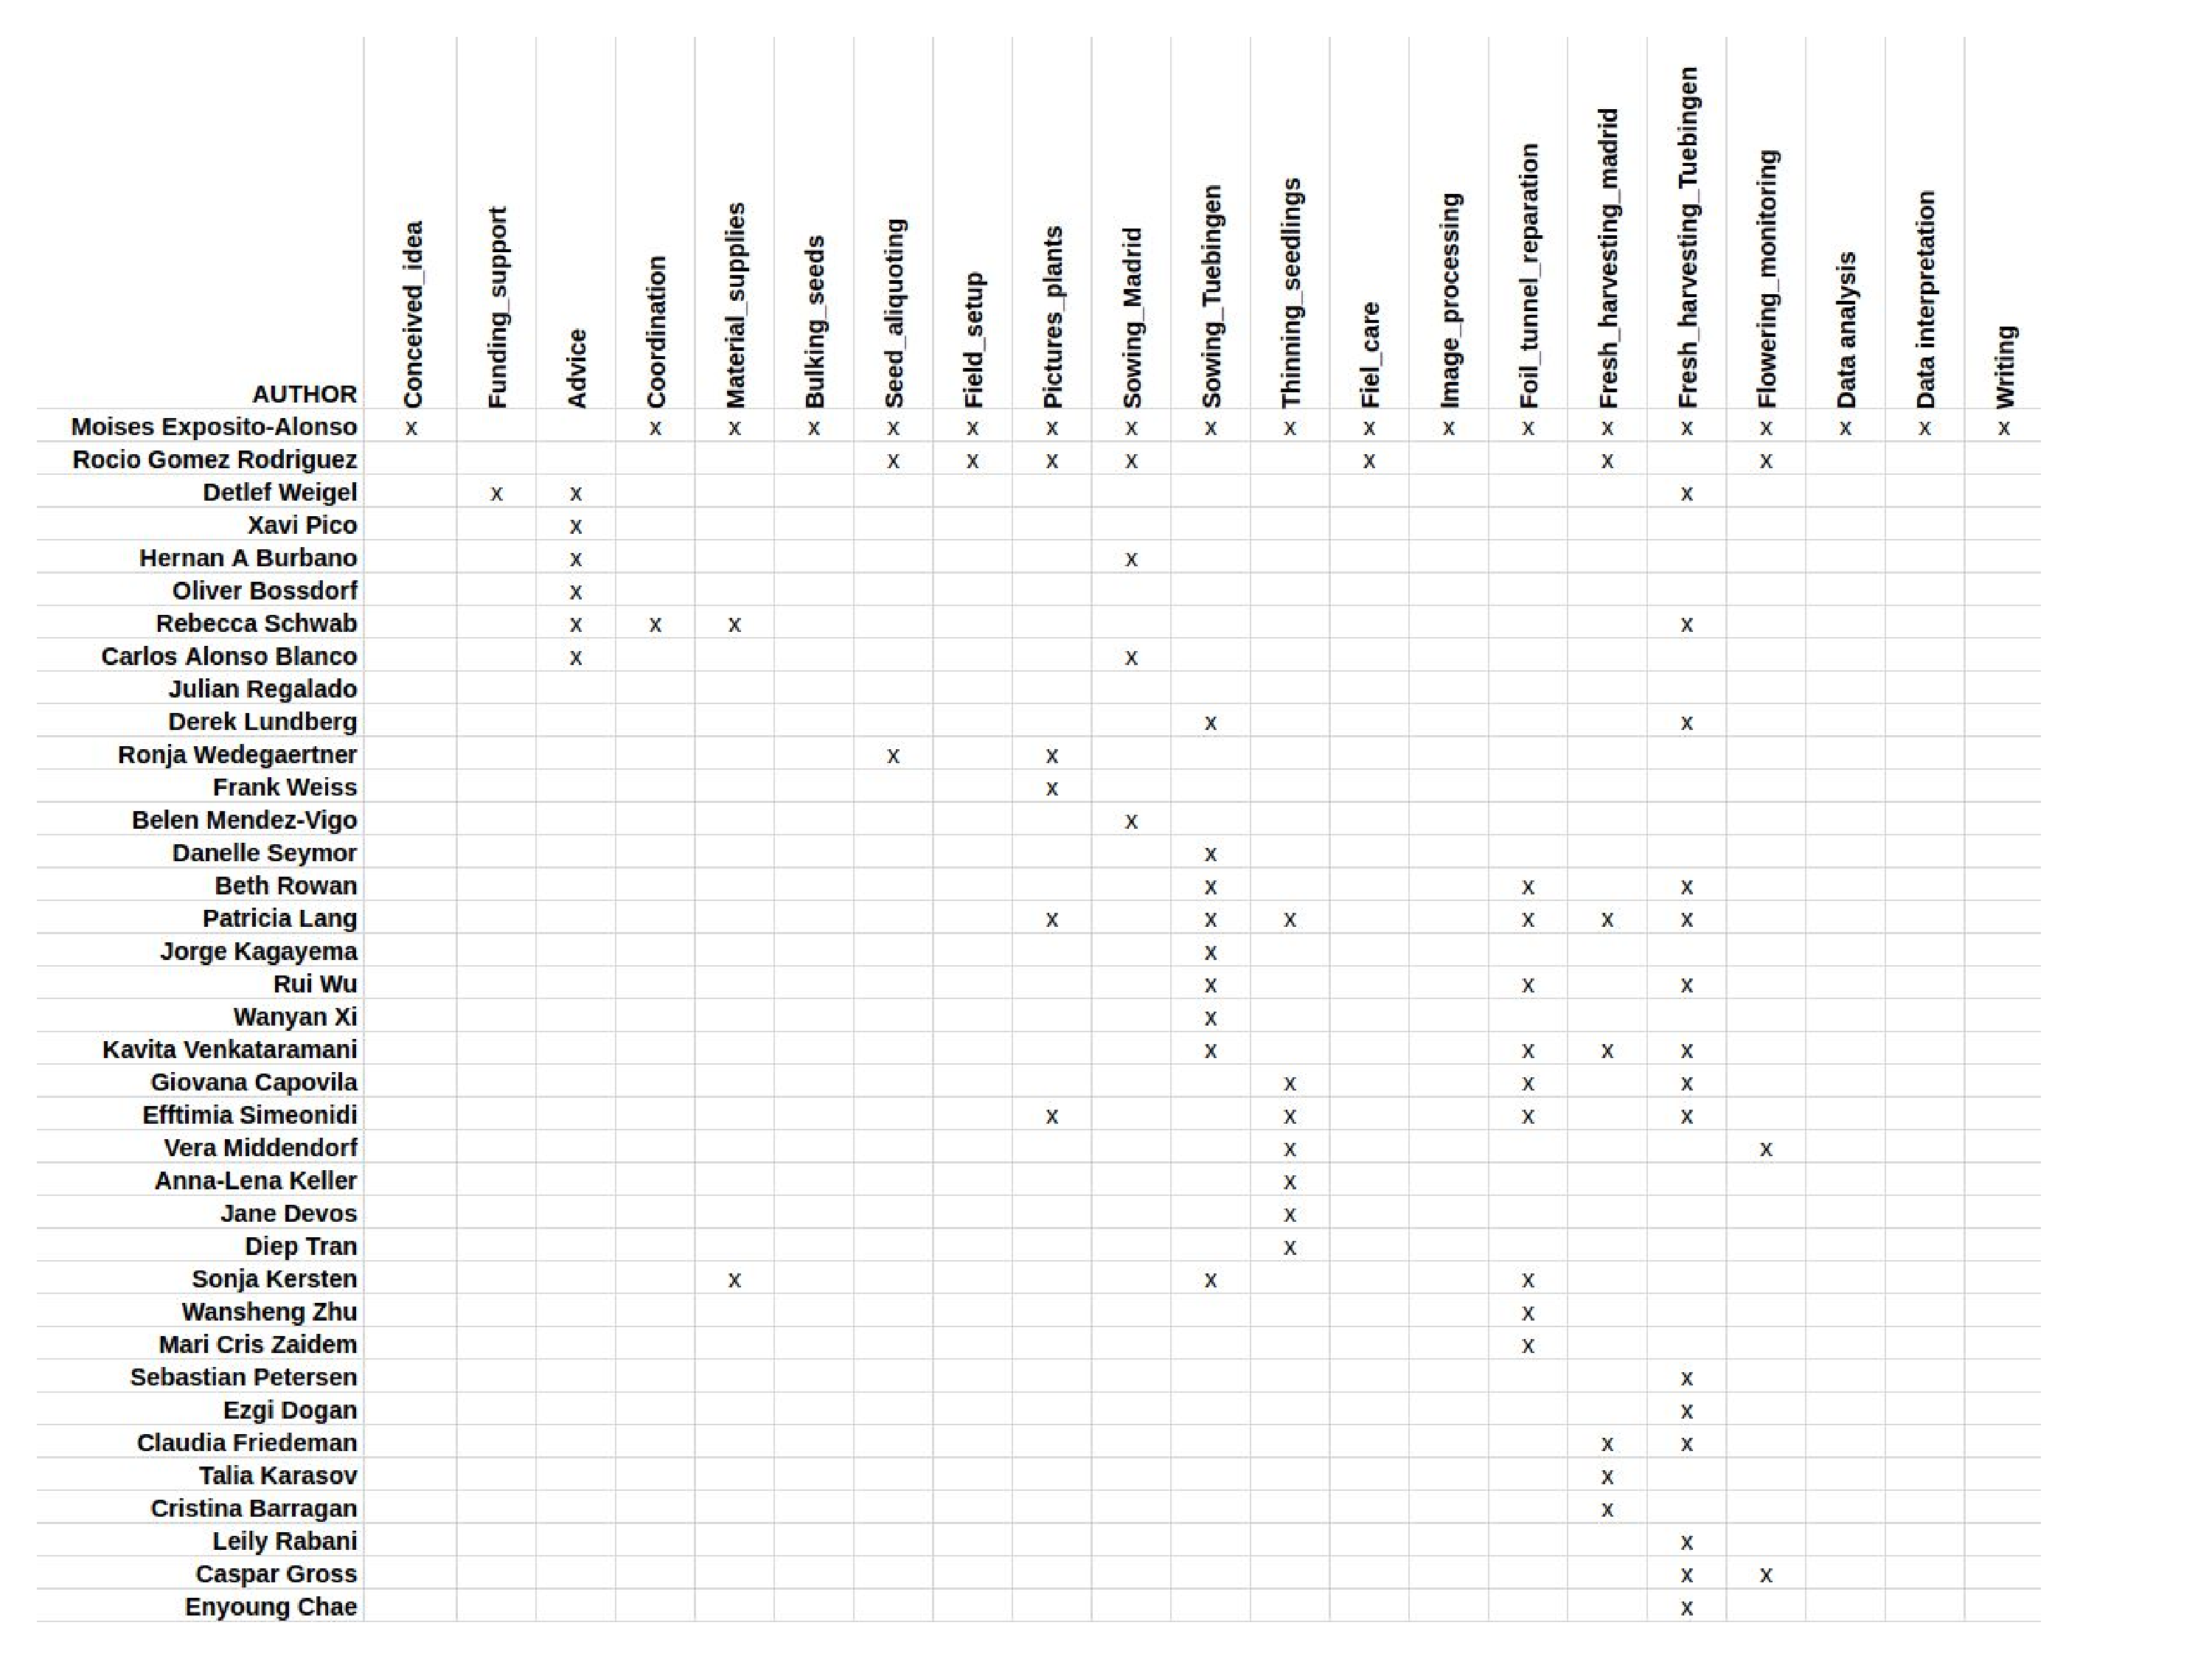
\includegraphics[width=7in]{../figs/Figure_people_contribution.pdf.png}}

\section{References}\label{references}


\end{document}
